% !TeX program = pdflatex
\documentclass[tikz,border=8pt]{standalone}
\usepackage{tikz}
\usetikzlibrary{angles,quotes,positioning}
\definecolor{FigureBlue}{HTML}{2563EB}
\definecolor{FigureOrange}{HTML}{EA580C}
\begin{document}
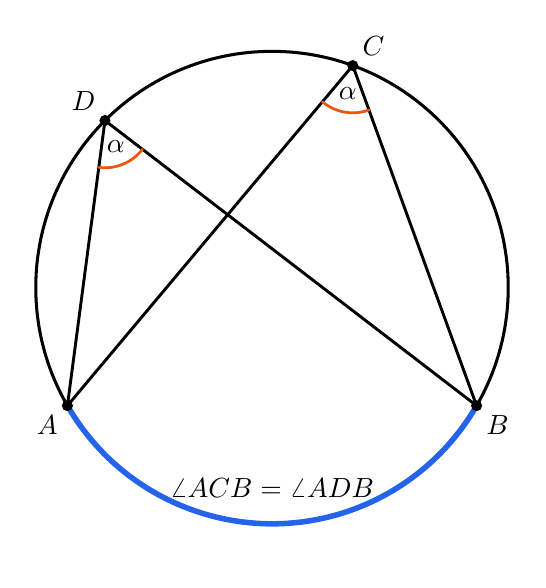
\begin{tikzpicture}[line cap=round,line join=round]
  \coordinate (O) at (0,0);
  \coordinate (A) at (210:3);
  \coordinate (B) at (330:3);
  \coordinate (C) at (70:3);
  \coordinate (D) at (135:3);

  \draw[line width=1.1pt] (O) circle (3);
  \draw[FigureBlue,line width=2pt] (A) arc[start angle=210,end angle=330,radius=3];
  \draw[line width=1.05pt] (A)--(C)--(B) (A)--(D)--(B);
  \pic[draw=FigureOrange,line width=1pt,angle radius=6mm,"$\alpha$"] {angle=A--C--B};
  \pic[draw=FigureOrange,line width=1pt,angle radius=6mm,"$\alpha$"] {angle=A--D--B};

  \foreach \P in {A,B,C,D}{\fill (\P) circle (2pt);}
  \node[below left] at (A) {$A$};
  \node[below right] at (B) {$B$};
  \node[above right] at (C) {$C$};
  \node[above left] at (D) {$D$};
  \node[below=8mm] at (O |- A) {$\angle ACB=\angle ADB$};
\end{tikzpicture}
\end{document}
